% document style
\documentclass{book}

% complex image tool
\usepackage{tikz}

% coordinate calculations
\usetikzlibrary{calc}

%\usetikzlibrary{positioning}

% --
% document

\begin{document}

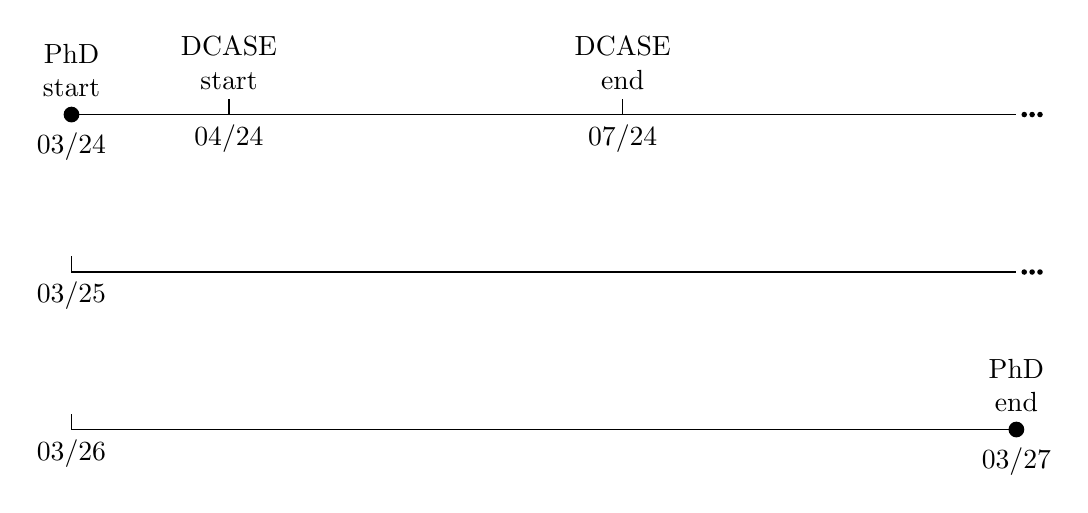
\begin{tikzpicture}
  
  % coordinates
  \coordinate (start_point) at (0, 0);
  \coordinate (dcase_start) at (2, 0);
  \coordinate (dcase_end) at (7, 0);
  \coordinate (end_point) at (12, 0);

  % start point
  \node at (start_point) (start_point_node) [circle, fill=black, inner sep=0mm, minimum size=2mm] {};
  \node at (start_point_node.north) (sp1) [anchor=south, align=center] {PhD\\start};
  \node at (start_point_node.south) (sp2) [anchor=north, align=center] {03/24};

  % dcase
  %\node at (start_point) (dcase_start) {};
  \draw (dcase_start) -- ++(0, 2mm);
  \node at (dcase_start.north) [anchor=south, align=center, yshift=2mm] {DCASE\\start};
  \node at (dcase_start.south) [anchor=north, align=center] {04/24};

  \draw (dcase_end) -- ++(0, 2mm);
  \node at (dcase_end.north) [anchor=south, align=center, yshift=2mm] {DCASE\\end};
  \node at (dcase_end.south) [anchor=north, align=center] {07/24};

  % end
  %\draw (end_point) -- ++(0, 2mm);
  %\node at (end_point.south) [anchor=north, align=center] {03/25};

  % line 
  \draw (start_point) -- (end_point);

  % ...
  \fill (end_point) [xshift=1mm] circle (1pt);
  \fill (end_point) [xshift=2mm] circle (1pt);
  \fill (end_point) [xshift=3mm] circle (1pt);


  % --
  % second timeline

  % relative coordinates
  \coordinate (second_timeline_start) at ($ (start_point) + (0, -2cm) $);
  \coordinate (second_timeline_end) at ($ (start_point) + (12, -2cm) $);

  \draw (second_timeline_start) -- (second_timeline_end);

  % start
  \draw (second_timeline_start) -- ++(0, 2mm);
  \node at (second_timeline_start.south) [anchor=north, align=center] {03/25};

  % end
  %\draw (second_timeline_end) -- ++(0, 2mm);
  %\node at (second_timeline_end.south) [anchor=north, align=center] {03/26};

  % ...
  \fill (second_timeline_end) [xshift=1mm] circle (1pt);
  \fill (second_timeline_end) [xshift=2mm] circle (1pt);
  \fill (second_timeline_end) [xshift=3mm] circle (1pt);

  % --
  % third timeline

  % relative coordinates
  \coordinate (third_timeline_start) at ($ (start_point) + (0, -4cm) $);
  \coordinate (third_timeline_end) at ($ (start_point) + (12, -4cm) $);

  \draw (third_timeline_start) -- (third_timeline_end);

  % start
  \draw (third_timeline_start) -- ++(0, 2mm);
  \node at (third_timeline_start.south) [anchor=north, align=center] {03/26};

  % end point
  \node at (third_timeline_end) (end_point_node) [circle, fill=black, inner sep=0mm, minimum size=2mm] {};
  \node at (end_point_node.north) [anchor=south, align=center] {PhD\\end};
  \node at (end_point_node.south) [anchor=north, align=center] {03/27};

\end{tikzpicture}

\end{document}